\documentclass[a4paper, 10pt]{article}

\usepackage[siunitx]{circuitikz}
\usepackage[margin = 1in]{geometry}
\usepackage{rotating}
\usepackage{ifthen}

\usetikzlibrary{intersections}

\def\cornerhypo{0.15}
\def\cornerbase{0.4cm}
\def\cV{|-}
\def\cH{-|}

\newcommand\constcorner[2] {
    coordinate (curtmp)
    #2 coordinate (FinalCornerTmp)

    (curtmp#1FinalCornerTmp) coordinate (LastCornerTmp)
    ($(LastCornerTmp)!\cornerbase!0:(FinalCornerTmp)$) coordinate (sectmp)
    ($(LastCornerTmp)!\cornerbase!0:(curtmp)$) coordinate (fsttmp)

    (curtmp) -- (fsttmp) -- (sectmp)
    coordinate (FinalCornerTmp)
}


\newcommand\corneranticlk[1] {
    coordinate (curtmp)
    #1 coordinate (LastCornerTmp)

    ($(LastCornerTmp)!\cornerbase!90:(curtmp)$) coordinate (sectmp)
    ($(LastCornerTmp)!\cornerbase!0:(curtmp)$) coordinate (fsttmp)
    (curtmp) -- (fsttmp) -- (sectmp)
}

% \ctikzsubcircuitdef{msFlop} {EC, IEC, D, RST, Q} {
\ctikzsubcircuitdef{test} {EC} {
    coordinate(#1-EC)
    \corneranticlk {++(0,4)}
    \corneranticlk {++(4,0)}
    -- ++(4,0)
}

\tikzset{fulladder/.style = {muxdemux, muxdemux def = {
    NL = 3, NR = 3, NB = 0, NT = 0,
    Lh = 3, Rh = 3,
    w = 5
    },
    draw only right pins = {1, 3}
    }
}

\tikzset{logicop/.style = {muxdemux, muxdemux def = {
    NL = 3, NR = 1, NB = 0, NT = 0,
    Lh = 3, Rh = 3,
    w = 5
    },
    }
}

\def\fulladdername{\texttt{ADDER}}
% \def\logicopstyle{\texttt{}}


% \tikzset{fulladder/.style = {muxdemux, muxdemux def = {
%     Lh = 3, NL = 3, Rh = 3, NR = 3, NB = 0, w = 6, NT = 0 },
% draw only right pins = {1, 3}}
% }

% \ctikzsubcircuitdef{onebitalu} {ina, inb, eclk, ieclk, rst, op0, op1, op2, regout, aluout} {
\ctikzsubcircuitdef{onebitalu} {L} {
    coordinate (#1-L)
    node [fulladder] (#1-flad) {\fulladdername}
}


\ctikzsubcircuitactivate{test}
\ctikzsubcircuitactivate{onebitalu}


\newcommand\wow[2] {
    \draw [gray] (0,0) -- ++(1,1) coordinate (tmp);

    \draw (tmp) \test{#1}{#2};
}

\begin{document}

\section{1 bit ALU}

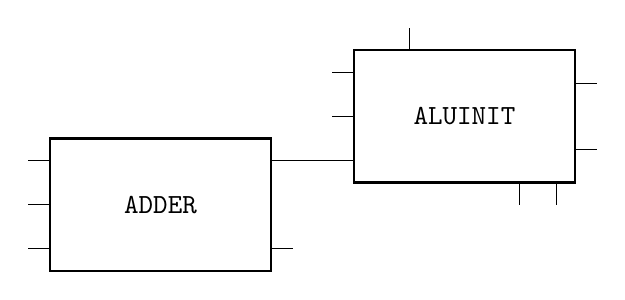
\begin{tikzpicture}[american]

    %  % \ctikzset{muxdemuxes/thickness = 3, multipoles/external pins thickness = 1.5, bipoles/tline/width = 3}

    %  \draw[semithick]

    %  node [muxdemux, rotate = -90, muxdemux def = {NL=10, NR=3, NT=0, NB=4,
    %  w = 2.5, Lh = 10, Rh = 6.5, inset Lh = 3.5, inset w = .75, inset Rh = 1.75,
    %  square pins=1
    %  },
    %  draw only left pins={2-9},
    %  draw only right pins={1-2},
    %  draw only bottom pins={2-4}]
    %  (mux) {
    %      \begin{turn}{90}
    %          \texttt{MUX8}
    %      \end{turn}
    %  }

    %  % (mux.rpin 3) -- ++(1,1)
    %  ;

    % \tikzset{blockdef-above/.style={
    %     {Straight Barb[harpoon, right, length=-0.2cm]}-{Straight Barb[harpoon, left, length=-0.2cm]},
    %     black,
    %     }}

    \tikzset{barbarrow/.style = {> = {Straight Barb[right, length = 5pt, width = 5pt]}}}


    \tikzset{testing/.style = {muxdemux, muxdemux def = {
        NL = 3, NR = 2, NB = 0, NT = 0,
        Lh = 3, Rh = 3,
        % Lh = 5.35, Rh = 3,
        w = 5
    },
    }
    }

    \tikzset{aluInit/.style = {muxdemux, muxdemux def = {
        NL = 3, NR = 2, NB = 6, NT = 2,
        Lh = 3, Rh = 3,
        % Lh = 5.35, Rh = 3,
        w = 5
    },
    draw only top pins = {1},
    draw only bottom pins = {5, 6},
    }
    }


    \draw
    (0,0)
    node (flad) [fulladder, anchor = lpin 1]{\texttt{\fulladdername}}
    (flad.rpin 1) -- ++(0.5,0)
    node (ainit) [aluInit, anchor = lpin 3]{\texttt{ALUINIT}}

    ;



\end{tikzpicture}

\begin{circuitikz}[american]

    \tikzset{barbarrow/.style = {> = {Straight Barb[left, length = 5pt, width = 5pt]}}}

    \draw
    (0,0) -- ++(1,1)
    \test {hai} {EC}
    ;

\end{circuitikz}

\begin{circuitikz}[american]
    \draw

    (0,0)
    coordinate (start)
    \constcorner {\cH} {++(1.5,-1)}
    (LastCornerTmp) ++(0,-1.5) coordinate (tmp)
    (FinalCornerTmp) -- (tmp)
    \constcorner {\cV} {++(-1,-1.5)}
    (LastCornerTmp) ++(-1.5,0) coordinate (tmp)
    (FinalCornerTmp) -- (tmp)
    \constcorner {\cH} {++(-1.5,1)}
    (LastCornerTmp) ++(0,1.5) coordinate (tmp)
    (FinalCornerTmp) -- (tmp)
    \constcorner {\cV} {++(1,1.5)}
    -- (start)
    ;
\end{circuitikz}

\end{document}
